% !TEX root = ../master-thesis.tex

% tweezer_loading.tex
% \subsection{x Tweezer loading} \label{subsec:tweezer-loading}




\begin{figure}
    \centering
    \addletter{90}{a}
    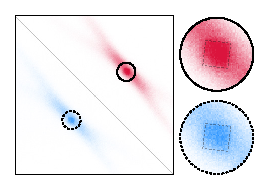
\includegraphics{fig-ai/loading-from-odt-1-ai.pdf}
    \phantom{42}
    \addletter{90}{b}
    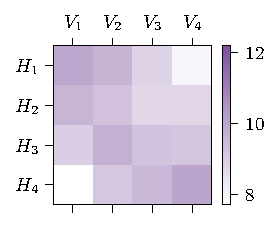
\includegraphics{fig-py/loading-from-odt-2.pdf}
    \phantom{42}
    \addletter{90}{c}
    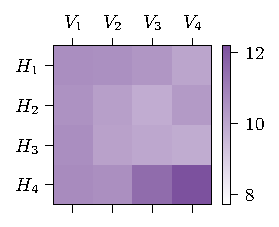
\includegraphics{fig-py/loading-from-odt-3.pdf}
    \caption[Inhomogeneous loading from ODT to tweezer arrays]{
    \textbf{Inhomogeneous loading from ODT to tweezer arrays.}
    (a) Atom distribution for a $6\times6$ array (averaged over 10 realizations), demonstrating inhomogeneous loading from the optical dipole trap (ODT).
    (b) Observed atom number distribution for a uniformly powered $4\times4$ tweezer array, revealing systematically lower loading efficiency at corners (averaged over 30 realizations).
    (c) Improved uniformity after manual adjustment of tweezer intensities, specifically enhancing corner powers (averaged over 30 realizations).
    }
    \label{fig:loading-from-odt}
\end{figure}

% \textbf{Tweezer loading}.
Understanding and characterizing atom loading from the ODT into tweezer arrays is crucial for achieving high-fidelity deterministic state preparation, as loading inhomogeneities directly impact the reliability of doublon creation. Even with perfect balancing of tweezer intensities, residual imperfections inevitably persist in the final atom distributions. These imperfections arise from several distinct contributions, including tweezer movements, loading processes from the ODT, and fluorescence imaging. The present subsection specifically examines the influence of loading atoms from the ODT into the tweezer array, isolating this particular contribution from other experimental stages.

% % \textbf{Tweezer loading}.
% Even with perfect balancing of tweezer intensities, residual imperfections inevitably persist in the final atom distributions. These imperfections arise from several distinct contributions, including tweezer movements, loading processes from the optical dipole trap (ODT), and fluorescence imaging. The present subsection specifically examines the influence of loading atoms from the ODT into the tweezer array, isolating this particular contribution from other experimental stages.

% \textbf{Characterization of atom loading from the ODT.}
To systematically investigate loading effects, atom numbers in individual tweezers are measured directly after the evaporation stage and prior to spilling. At this intermediate stage, the number of atoms per tweezer is inferred from the fluorescence signals recorded by the nuvu camera. Combining previously obtained calibration data from step plots and single-atom counting experiments (Sec.~\ref{sec:imaging}), approximately 30 photons per atom are expected to be detected by the camera, allowing quantitative estimation of atom populations per tweezer.

% \textbf{Constraints on minimal inter-tweezer spacing.}
In the current setup, the minimum feasible spacing between tweezers is restricted to approximately $5\,\mu$m. Attempts to further reduce this separation consistently resulted in elevated atom losses, presumably due to parametric heating effects associated with closely spaced potentials. Although stroboscopic methods—rapidly alternating between different AOD configurations—might mitigate these heating effects, such approaches require further systematic investigation and remain topics for future research. A dedicated characterization of minimal achievable spacing and associated atom retention rates is necessary and will be addressed in forthcoming studies.
 % \red{(add plot on the minimum distance between atoms in future)}.

% \textbf{Dragging approach for enhanced loading.}
A preliminary investigation explored an alternative strategy: the dragging method, in which an array of tweezers is adiabatically translated through the ODT during loading. This approach allowed loading of larger tweezer arrays compared to the stationary loading method. However, despite its promise, the dragging method exhibited potential heating issues both in the ODT reservoir and within the tweezers themselves. The effectiveness of dragging critically depends on an accurate balance between tweezer and ODT depths, and careful optimization of these parameters also remains a necessary direction for future research.

% \textbf{Observed inhomogeneity in tweezer loading.}
With stationary loading at a fixed $5,\mu$m spacing, systematic spatial inhomogeneities are consistently observed, particularly affecting the corner regions of the tweezer array. This effect is illustrated clearly in Fig.\ref{fig:loading-from-odt}a, which shows an averaged atom distribution for a $6\times6$ tweezer array directly after loading from the ODT. Atom occupancy at corner sites is markedly reduced relative to central sites. A quantitative assessment of loading imbalance is provided in Fig.\ref{fig:loading-from-odt}b, depicting the measured atom number distribution for a uniformly powered $4\times4$ tweezer array. The corners show systematically lower populations compared to central positions.

% \textbf{Improvement via manual intensity adjustments.}
To overcome this intrinsic loading imbalance, a manual redistribution of tweezer intensities was performed using the previously measured camera-based crosstalk matrix. Specifically, the intensities of corner tweezers were deliberately increased relative to central tweezers to compensate for the lower initial loading rates. This simple yet effective manual intervention improved corner loading significantly, increasing atom numbers at corner positions by approximately 20\% as demonstrated in Fig.~\ref{fig:loading-from-odt}c. Consequently, this intensity adjustment facilitated more homogeneous atom distribution and higher fidelity in subsequent state preparation procedures.

In summary, careful analysis and targeted intensity adjustments during the ODT loading phase substantially reduce residual inhomogeneities in atom occupancy. However, further improvements and more systematic methods—including minimal spacing optimization, stroboscopic techniques, and dragging approaches—represent valuable areas for continued research.

